\section{Introduction}
\label{sec:introduction}

Spatial partitions represent physical structures by assigning regions to their constituent objects. In polycrystalline materials, these regions describe grain shapes and neighbor relations \cite{Spettl2016,BournePearceRoper2025}. In molecular structures, atomic regions are used to estimate volumes and packing \cite{Richards1974}, or to assign electron populations \cite{Bader1990}. Simple geometric models describe these regions through a small set of parameters, which must be chosen from the available information about the structure.

A simple model is the ordinary Voronoi diagram. Given distinct points $p_1,\ldots,p_n$ in Euclidean space $\mathbb R^d$, called \emph{sites}, the cell of each site consists of the points no farther from it than from any other site \cite{Okabe2000}. The cells cover space and may share boundary points. For two sites, their dividing hyperplane is perpendicular to the line joining them and passes through its midpoint. With the sites fixed, this construction offers no freedom to adjust the division.

A \emph{power diagram}, also called a Laguerre diagram, adds one real scalar weight $w_i$ to each site \cite{Aurenhammer1987}. It assigns points by comparing the \emph{power distances}
\[
\pi_i(x)=\|x-p_i\|^2-w_i.
\]
The power cell of a site contains the points where its power distance is minimal. Equal weights recover the ordinary Voronoi diagram. Equality of the power distances for two sites defines a hyperplane, which we call their \emph{pairwise separator}. Changing the weight difference translates this plane along the line through the sites without changing its orientation. Figure~\ref{fig:two-site-separators} shows how increasing $w_j$ moves the separator toward $p_i$, enlarging the cell of $p_j$. Thus weights allow the division to change while preserving the site positions, although the cell boundaries remain piecewise planar.

\begin{figure}[tbp]
\centering
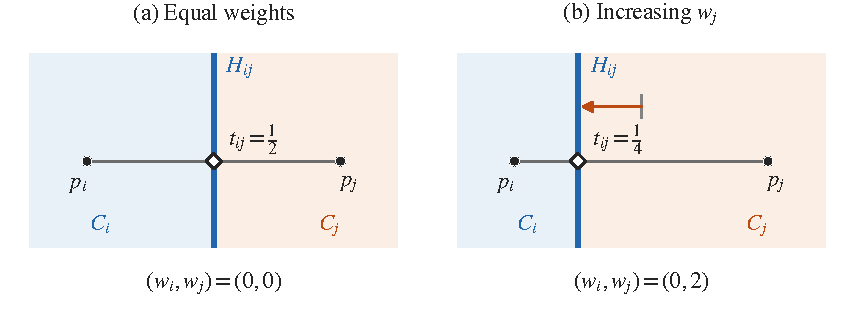
\includegraphics[width=\linewidth]{figures/figure_02_separators.pdf}
\caption{Two fixed sites with equal and unequal weights. (a) Equal weights give the ordinary Voronoi boundary at the midpoint. (b) Increasing $w_j$ moves the boundary toward $p_i$ and enlarges the cell of $p_j$. Both panels use the same sites and scale. With only two sites, the entire pairwise separator is a shared boundary.}
\label{fig:two-site-separators}
\end{figure}

Choosing parameters from observations gives an inverse problem whose form depends on what is known about the desired partition. Duan et al.\ recover site positions and weights from a supplied Laguerre tessellation \cite{Duan2014}. Spettl et al.\ fit a Laguerre approximation to segmented tomographic images, minimizing squared distances from interface samples to pairwise separating planes while varying both site positions and radii \cite{Spettl2016}. Bourne, Pearce and Roper instead recover or fit tessellations from cell volumes and centroids using optimal transport \cite{BournePearceRoper2025}.

Other constructions prescribe which cells must meet. Alexa computes weights at fixed sites, when feasible, so that selected cells have a common intersection, producing meshes that contain prescribed edges or triangles \cite{Alexa2020}. Related methods permit additional sites and subdivisions of the prescribed elements \cite{Bogiokas2025}. In these constructions, the required intersections are part of the input; they need not follow from a fit to measured boundary locations.

We study a setting in which the sites are fixed and the inputs are numerical dividing positions for selected pairs. The positions may be inferred from interface samples or predicted independently, without a supplied global partition. For example, atomic density profiles can predict a dividing position along the line through two nuclei without assigning the rest of space to either atom. The nuclear coordinates specify the molecular geometry, so retaining them is part of the modeling task. We seek one set of site weights that reconciles these local positions. For a given pair, the fixed sites determine the orientation of its separator; one coordinate on the full line through them specifies its position and hence a desired weight difference. Observations may be missing, repeated or noisy.

One weight participates in every observation involving its site, so independently chosen separator positions can impose conflicting requirements. We represent sites by graph vertices and observations by edges. Around a closed chain of observations, the signed weight differences must sum to zero. If compatible observations connect all sites, they determine the weights up to a common shift that leaves the diagram unchanged. When observations conflict, weighted least squares reconciles them through a classical graph-Laplacian problem \cite{Jiang2011}. For interface samples, this quadratic fit is also the fixed-site form of Spettl et al.'s interface discrepancy, with their squared radii identified as weights \cite{Spettl2016}.

Agreement with the pairwise positions does not ensure that the corresponding cells share a face. On a pairwise separator, the two power distances are equal; yet at every point some other site may have a smaller power distance. Even if a common face exists, it may lie away from the line through the pair. We therefore check both the realized faces and whether they contain the separator's intersection with the site line. Fitting the separator positions and assessing their geometric realization are separate steps.

We develop compatibility and identifiability conditions for these observations, together with fitting formulations for noisy data and hard bounds on separator positions. When the line--plane intersection lies inside a face, its distance to the face boundary, measured within the separator plane, defines \emph{centered clearance}. For fixed, unconstrained least-squares problems in finite nonperiodic configurations, perturbation bounds connect changes in the observations to stability of the local test. A computational workflow combines fitting, diagram construction and face checking, including periodic systems, and is implemented in \texttt{pyvoro2} \cite{Pyvoro2_063}.

Synthetic experiments test recovery from exact compatible data and the effects of missing observations, noise and model mismatch. An application to 100 molecules compares predictions from atomic density profiles, their fitted separators and the resulting pair relations with a reference derived from the Quantum Theory of Atoms in Molecules (QTAIM) \cite{Bader1990}. The experiments show that closer agreement with imposed local targets need not improve agreement with an independent reference. In the molecular tests, clearance helps distinguish reference contacts among nonbonded faces that pass the local test. These comparisons concern separator positions and pair relations; complete atomic basins are not reconstructed \cite{PowerfitArchive2026}.

Sections~2--4 develop the observation model, graph fitting and geometric assessment. Section~5 describes the computational workflow. Sections~6 and~7 present the synthetic experiments and molecular application, followed by discussion and conclusions in Sections~8 and~9. The appendices contain supporting arguments, geometric qualifications, and implementation and experimental protocols.
